\documentclass[conference]{IEEEtran}

\usepackage{graphicx}

% correct bad hyphenation here
\hyphenation{}

\begin{document}
% paper title
% can use linebreaks \\ within to get better formatting as desired
\title{Evolution and Challenges in testing of security on ICS/SCADA System after Stuxnet}

% author names and affiliations
% use a multiple column layout for up to three different
% affiliations
\author{\IEEEauthorblockN{Atadjan Kurbanniyazov}
\IEEEauthorblockA{Department of Computer Science\\Faculty of Security Network and Systems\\University of Innopolis}
\and
\IEEEauthorblockN{Luis Funes}
\IEEEauthorblockA{Department of Computer Science\\Faculty of Security Networks and Systems\\University of Innopolis}} 

% make the title area
\maketitle

\begin{abstract}
Industrial control systems run 24/7 and 365 to  control and monitor industrial and infrastructure processes. There is a lot of security flaws and incidents, and challenges exist which can be solved with effective forensic simulations and investigation. This work describes potential threats, challenges, and investigations with potential issues and its solution, and shows us the limitations of traditional IT-based approaches, It presents for initiating continuous research in ICS  systems, especially on this incident.
Furthermore,  it discusses how the research community, third-party organizations, and vendors have tackled these serious barriers and problems so far.
    
\end{abstract}

\IEEEpeerreviewmaketitle

\section{Introduction}
Eight years after the Stuxnet was undiscovered and a targeted cyberattack against the Iranian nuclear program, both the United States and Israel were threatened by the prospect of an Iranian breakout towards nuclear weapons production. After all, should we anticipate another cyber attack against Iran?

  Industrial control systems (ICS) surround us and we have not even mentioned it: they have used in electric, water and waste-water, nuclear, oil and gas industries, transportation, chemical, pharmaceutical, constructions, food and beverage, and manufacturing plants (e.g., automotive, aerospace, and durable goods). Smart cities, houses, and self-driving cars, medical equipment,  – all of that is managed by ICS.
If a control system is deployed in the local area and can supervise and control its individual components, it is called a supervisory control and data acquisition system [1]. The differences between SCADA and ICS in that two terms are frequently used interchangeably by the professional, engineers in the field of industrial control systems. It encompassing to large geographically distributed areas, where is possible to find pipelines for gas systems also the distribution of electricity or water. ICS is the correct terminology to use, but only speaking about the industrial automation.

It is also helpful to use both terms together because the term SCADA is actually better known in the professional media, among journalists, civils workers, and the public. SCADA in point of fact is a discipline within ICS. However,  it some new term naming use the term  'SCADA' in this paperwork to identify all kinds of control  systems, which is the same as ICS or SCADA, but there is no difference in it.  
In the deployment of ICS/SCADA  systems, it was intended to run as isolated networks, specific security mechanisms. It was used as a simple point-to-point Modbus protocol, which has become a standard for RTU and
PLC communications, just sending bit 0 or 1. During communication on a Modbus network, the protocol determines the way to communicate with each controller device depending on its address, recognize a determined message addressed to it and then taken the corresponding action finally extract any information or data attached to it.  They have consisted of  
input or terminal units.  Due to advances of info-communications technologies,  they and adopted
new technologies  (such as wireless  IP communication, satellite, LTE, 4G).  In recent years, most of the advanced SCADA changed to communicate over public  IP  networks, through virtual private networks [2], order to be seamlessly integrated to  SCADA external information, e.g. corporate mail  systems, weather data. Due to business needs and the reachability and reliability of SCADA  systems from which depends mainly on the wider  network, brings threats also that were unimagined at the time when those systems were persuaded. Vendors, asset owners, and third parties organizations in the past ten years, address it by means of
security mechanisms, processes, standards, and regulation [3].   
The finding of Stuxnet in 2010 was an additional mystery and change the security policy for ICS/SCADA owners, vendor suppliers, and operators.  During the long investigation, this malware that is specifically written to attack automation system and have infected an estimated 100,000 computers and servers around the world[4]. 
More recently, another malware 
has  been  discovered  that  is  an espionage  tool  and is considered    an
other tools that more sophisticated than Stuxnet [5].
To further understand the content of this paper, we must also describe what for was this worm created, its purpose, its effects, damage and how it spreads with plain simulation on infecting new version of the software.

	In the following sections we will present and analyze a worm, and with some known application, in sections  \ref{sec:CT} and III respectively . In section VI, we will mention some investigation countermeasures in order to protect a system from potentially harmful malware and worm.

\section{History of different vulnerabilities in ICS/SCADA}
\label{sec:CT}
In this section, we will highlight the infrastructure of ICS and vulnerabilities from the past attacks which infected other systems.
Only a few examples will be exposed, and its selection was based on their usage and exploit frequency.
\subsection{Typical infrastructure of ICS/SCADA}
For taking in account that upgrading or renew industrial control systems takes much longer time and much budget than upgrading traditional ICT systems and due to advance of technologies and data transfer, each industrial organizations have developed high-level ICS systems which mainly based on ICT technologies. However, due to demand of businesses and cost-effectiveness of productions which lead them to integrate these advanced technological systems into existing ISC infrastructure, for this occasion most of the organizations had to create additional telecommunication and information exchange path-media, mostly were unreliable and still prone to vulnerabilities. Most Industrial organizations believe that field-level information technologies will help to satisfy Confidentiality-Integrity-Availability (CIA) concept requirements and provide the telecommunication capabilities required to existing high-level information control systems and related IT infrastructure. The elements of ICS/SCADA system (given in Figure 1):
\begin{itemize}
   \item Stationary and portable systems (mostly computers, HMI) for operating and engineering staff
   \item ICS/SCADA monitoring servers, virtual servers, storages
   \item L2/L3 Industrial switches, routers and other devices
   \item Programmable Logic Controllers (PLC)
   \item Wireless devices (Antenna, relays, satellite telecommunications)
   \item Field devices of various levels of complexity and autonomy with digital or analog input/output
\end{itemize}
\begin{figure}[!htb]
	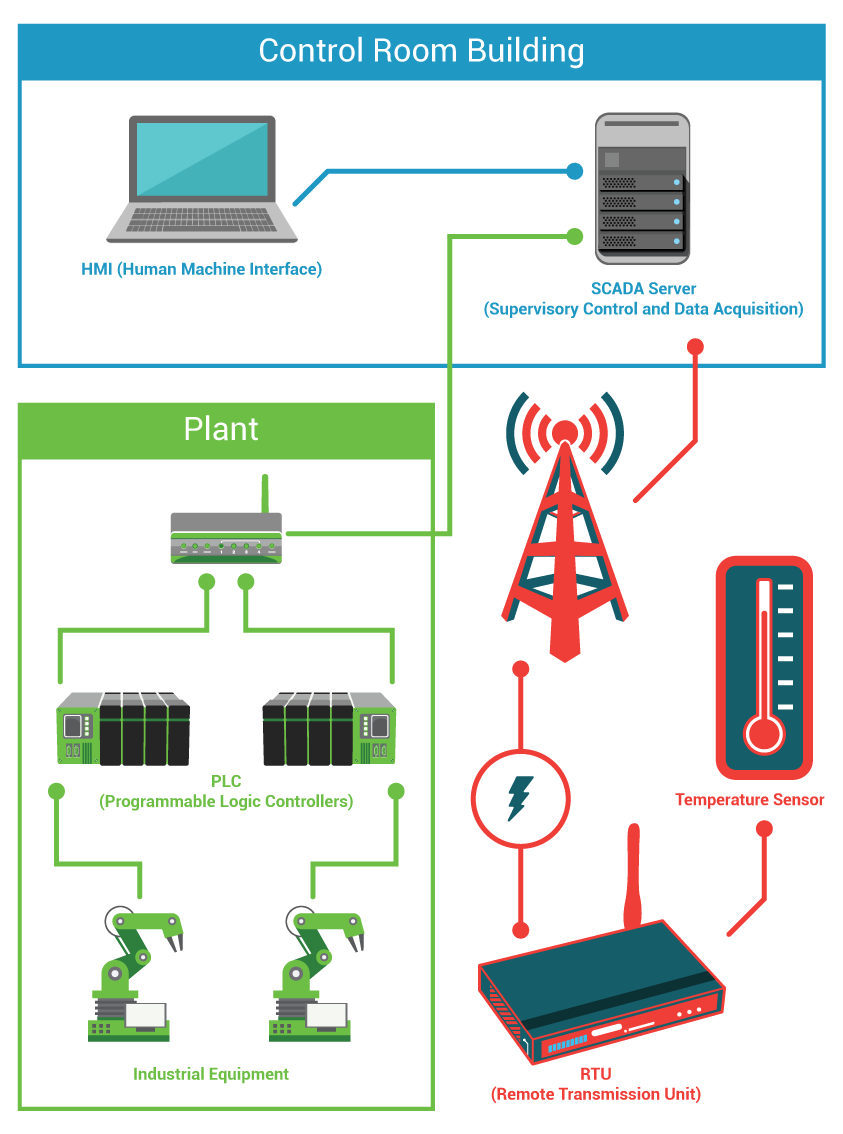
\includegraphics[width=0.49\textwidth]{images/SCADA5.png}
	\caption{ Chain of communication on ICS system}
	\label{fig:TCPIP}
\end{figure}
SCADA networks make use of specific and sometimes proprietary protocols. Many
of these protocols have known shortcomings that make them vulnerable to exploits and cyberattack.
Here are some examples:

MODBUS is an application-layer communication protocol. It provides client/server
communication between devices connected on different types of buses or networks.
It is mainly used for supervision and control of automation devices. The protocol is lack of security against unauthorized commands or interception of
data.

DNP3 (Distributed Network Protocol version 3) is a set of communication protocols used
between components of process automation systems. Its mainly used in electric and water companies. Although it was designed to be very reliable, but not designed to be secure from cyber attacks. It does not have any encryption, authentication or
authorization mechanism, the devices simply assume that all transferred data and messages are valid. All DNP3 attacks rely on the ability to intercept, modify or fabricate DNP3 data messages[6].



\subsection{Vulnerabilities}
The first officially published information on vulnerabilities in ICS systems and each component, dates back to 1997, when two vulnerabilities were published, the interruption in communications work of Worcester, Massachusetts Air Traffic Communications system,
vulnerabilities had significantly increased at that time. In Figure 2,  statistics show and proves to our result that over the past eight years, the number of attacks has increased
from nineteen vulnerabilities in 2010 to 189  in 2015. As we know that in a period of 2010-2015 there was a
period of significant growth in the number of vulnerabilities and cyber attacks against this type of systems, and reflecting the increased attention that
researchers and system vendors paid to the problem of ICS  security during this time.
By huge efforts by communities have  been superseded by a period of active research: every year 
150 vulnerabilities were detected, and the average amounts of ICS/SCADA vulnerabilities almost match this.

\begin{figure}[!htb]
	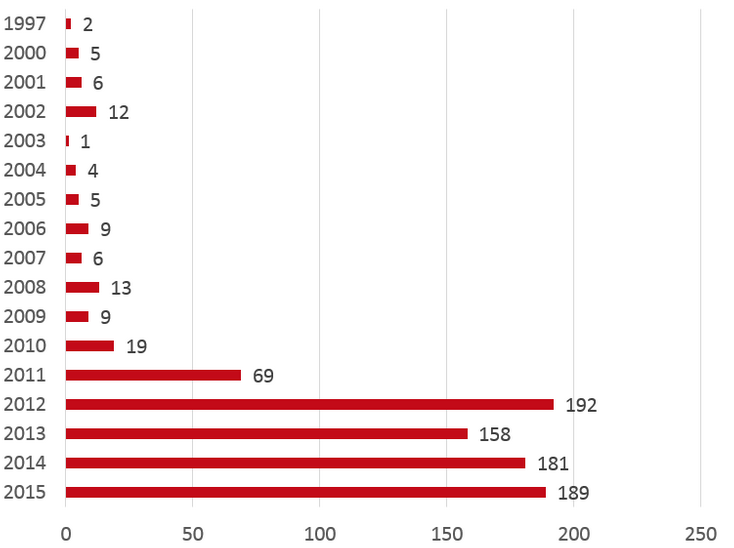
\includegraphics[width=0.49\textwidth]{images/scada2.png}
	\caption{  Attack on ICS system during decade}
	\label{fig:TCPIP}
\end{figure}
By last reports states that huge manufacturing facilities and critical infrastructures, such as energy sector and transportation, have fallen victim of targeted cyber attacks in recent years. The total loss which estimates about 300 million USD,  Maersk shipping company [3]and massive interruptions in production at Renault and Nissan plants [4] and a ransomware attack on the San Francisco public transit system[5] are only some of the examples that have appeared on headlines of the news.
.

\subsection{Preparation for Stuxnet}
The first mention about Stuxnet was appeared an article by security company VirusBlokAda from Belarus in June 2008 and named as "Rootkit. Tmphider". After that Microsoft confirmed that the worm was actively attacking systems running on Windows operating system which were managed and hosted ICS/SCADA systems and servers in different industries, manufacturing and production firms. But they did not give much attention to it and they even did not try to stop it. At that period of time, this worm exploited a Windows bug patches with Microsoft's update MS08-067. That bug was the same vulnerability used to devastating effect by the famous Conflicker worm in late 2008 and early 2009 that infected millions of machines.
\subsection{Windows exploits: Conficker}
On October 23, 2008, Microsoft published the CVE bulletin code of MS08-067, Vulnerability in Microsoft Server Service which allowed Remote Code Execution (RCE). Microsoft had explained that the vulnerability in the server services which lead for remote code execution when an affected server received a targeted  remote procedure call (RPC) request, and then  attackers  exploited these vulnerabilities without authentication by running arbitrary code on Windows 2000, SP2 and SP3, Windows Server 2003 SP1 and SP2, Vista Gold SP1, Windows Server 2008 and Windows 7 operating systems. 

Additionally, this exploit has been referred to as the Conficker virus, Downadup and Kido. Conficker was one of the fastest and largest worm infections. It was difficult to contain and control due to its use of many different advanced malware techniques. Conficker's code structure and logic include mechanisms to generate new domain names lists and it was difficult to search it in Internet points of redistributing data that the creators used for updates, command, and control of the infected hosts. Conficker uses binary validation procedures to validate signed updates by its creator. The use of binary encryption, digital signatures and advanced hash algorithms for its updates helped to control and hijack infected clients. This signed binary update mechanism allows them instant control of the millions of infected PCs worldwide.  Tracks of the worm were difficult and prevented its removal from host machines by obfuscating of its code. It was sophisticated that it could disable Windows systems security services, third-party firewalls, and anti-virus products, allowing systems to be in a vulnerable state which then lead to more infection and exploitation. In addition, it also blocked access to a site where you can download software for removing it, such as Symantec or McAfee.

\subsection{Windows exploit: Night Dragon}
Starting in November 2009, concentrated coordinating  and targeted attacks have been deployed against
oil, energy, and petrochemical sectors. It was involved with mechanism of social engineering, spear phishing
attacks, compromising and exploitation vulnerabilities of Microsoft Windows OS and  Microsoft Active
Directory, with use of remote administration tools (RATs) for intelligence and to theft of business information: operations, finance data, project plans . It was investigated that Night Dragon was originated primarily in China. Through
coordinated analysis of all events and tools used, McAfee had identified that many third parties organizations were involved to attack or had common interests.

\subsection{Windows exploit: Black Energy 3 2015}

\begin{figure}[!htb]
	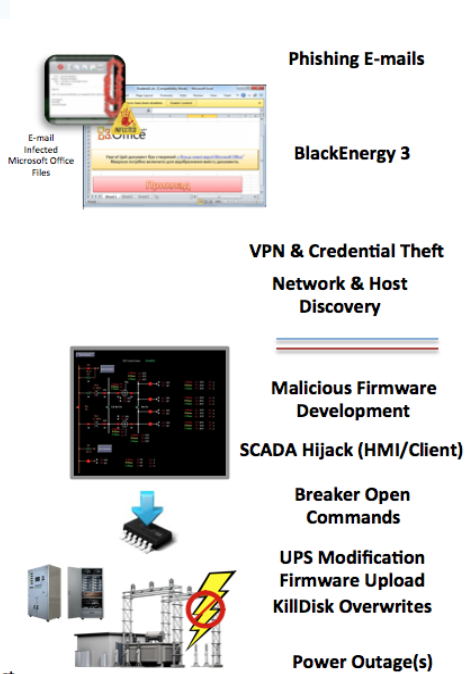
\includegraphics[width=0.49\textwidth]{images/KILLOFCHAIN.png}
	\caption{ Black Energy in ICS Kill Chain }
	\label{fig:TCPIP}
\end{figure}
 On December 23, 2015, the Ukrainian Kyivoblenergo, a regional electricity distribution company, reported service outages to customers. The blackout (electric power outages) were to a third party’s illegal entry into the company’s computer and ICS systems. It was investigated that this cyber attack impacted additional portions of the distribution power grid and forced operators to switch to manual mode, they have switched off the ICS system.

Thus the ICS distribution and management system was attacked and controlled remotely by foreign hackers. Resulting in several outages affecting 225,000 customers to lose power across some part of Ukraine. 



 How it was staged. The process of intrusion was staged in several parts of delivery, exploitation, and installation of the malicious Office documents which were delivered via email to local staff in the administrative or IT network of the electricity companies. When these documents
were opened, a pop-up message was displayed to users and for viewing document it just needed to enable the macros in the document as shown in Figure 3.

Enabling these macros allowed the malware to install BlackEnergy 3 exploit on the system after it connected to command and control IP addresses to enable communication by remote and the infected systems. These routes allowed hackers to gather information from the environment and enable access. It was under hackers control more than six months till attack on December 23, 2015.

\subsection{Windows exploit: Triton}
One year after this incident, the cybersecurity experts discovered another cyber attack on a safety instrumented systems, which was called as Triton or TRISIS. 
This tool was built with a lot of features, which includes the ability to read and write programs, individual functions and send queries for the state of the SIS controller. 
\begin{figure}[!htb]
	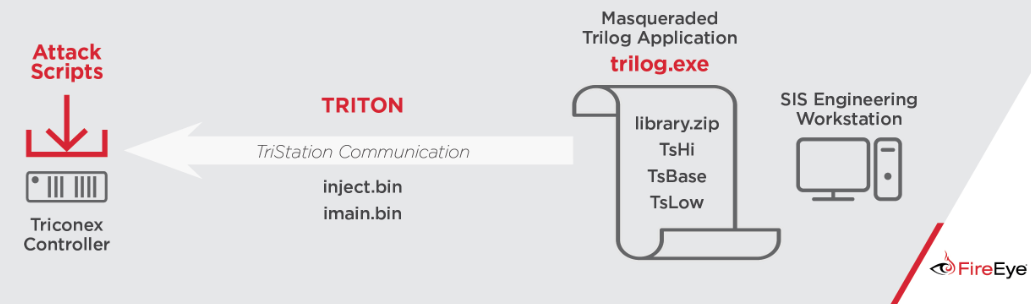
\includegraphics[width=0.49\textwidth]{images/Triton.png}
	\caption{ TRITON Architecture and Attack Scenario investigated by FireEye }
	\label{fig:TCPIP}
\end{figure}
Also it was mentioned that the TRITON malware could  communicate with Triconex SIS controllers (e.g. send  stop command or read its memory content) and could reprogram them remotely with an attacker-defined payload.  This payload left legitimate programs in place and expecting to continue operating without any fault or exception. If the controller failed to function, TRITON would attempt to restart it into a running state. If the controller did not recover within a defined period of time or timeout, this payload would overwrite the malicious program with invalid data to hide or erase its tracks.

Triton was deployed on an SIS engineering workstation running under Microsoft Windows operating system and it was named such way to masquerade as the legitimate Triconex Trilog application of Schneider Electric. This application was used for survey logs and was a part of the Schneider TriStation application suite, then Triton was delivered as a Py2EXE compiled python script file which was on a zip file, when running it by operators on station  then the  attacker-developed Triconex attack framework which interacted with the Triconex controllers on that station. Along with the executable files, it contained two binary files: 'inject.bin' (malicious function code) and 'imain.bin' (malicious control logic code),afterwards  they were deployed as the controller’s payload.

Trilog.exe used only an IP address to connect to the targeted Triconex device. It did not leverage the underlying TRITON library’s capability for Triconex device discovery, instead an instance of trilog.exe had to be called separately for each target controller in the environment. Once invoked, trilog.exe was checking the status of the controller, and then read the configuration information exposed by the TriStation protocol. If the control device was in a running state, trilog.exe encoded these payload files inject.bin and imain.bin and passed them to the communication libraries and then appended by controller’s program memory and its execution table[7].

After successfully inserting payloads to Triconex controller memory, the script started periodically check the status of the controller. If an error was detected, the communication library’s method SafeAppendProgramMod reeset the controller to the previous state using a TriStation protocol command. If this command failed, then it attempted to write to trilog.exe a small ‘dummy’ program to its memory. This technique was like an anti-forensics investigations in order to  hide the attacker hard-coded code on the Triconex controller.

Workflow of TRITON was implemented the TriStation protocol, which used by TriStation application, to configure controllers and use of three modules for exploit the infrastructure.

TsHi module is the high-level interface created by the malware’s authors that allows replicate operators to run attack scripts using the TRITON framework which used for reconnaissance and attack. Then accept binary data from the user, and handle the code ‘signing’ and check sums before to pass the data to lower level applications libraries  for serialization on to the local network.

TsBase module, another attacker-written module, contains the functions called by TsHi, which translate the attacker’s intended action to the appropriate TriStation protocol function code, it also packs and pads the data in to the appropriate format.

TsLow module is used for commuications in TriStation UDP wire protocol. The TsBase library depends on the ts\_exec method, which takes the function code and  response code, and serializes the commands payload over UDP. It checks the response from the control device against the expected values and returns back a resulting data structure indicating success or a False object representing failure[8].

\section{Investigate  structure  and  methods  of  exploitation   of   STUXNET   worm   and   how   it was spreading.}
\label{sec:IST}
	In this section we cover some investigation of malware and it is semantically structure and methods, which used for ICS  exploitation.
\subsection{ICS for ICT security challenges}
Cyber security challenges in industrial control networks are the result of rapidly increasing functional requirements and exponentially growing use of information technology in manufacturing and industrial environments. For past ten years, the raise of use automation systems has been closely connected with that of traditional ICT systems. An important requirement for industrial control systems is to persistent and permanent  availability of data of industrial processes. To meet business requirements, industrial control systems must evaluate modern functions that are not typical to ICT systems.



\subsection{Stuxnet Architecture}
Stuxnet is a complex piece of malware. Its
functioning in two
main "functions" mode: the propagation of the
virus, which is based upon the
vulnerabilities inherented in the Windows
platform, and the attack on ICS/SCADA
systems, which is focused on WinCC and
PLS.
Stuxnet could be the first advanced malware. It is thought that it was developed by the USA and Israel to attacking Iran's nuclear plants located in Natanz and disrupt whole nuclear program. It was attacked Windows systems using a zero-day exploit and  was focused on SCADA systems in order to  affect and damage the critical infrastructures in some spesific area of the world. It was spread from USB drivers. Also it was investigated that for making such massive attacks, need to have a team of highly motivated programmers with  knowledge of industrial processes and with their involving interests in the attacking industrial infrastructure in order to develop this malware.

 Kaspersky Lab  also investigated  that the sophisticated attack and was conducted with support from government. As it was investigated by Symantec   of the spreading of Stuxnet, which  says that  affected countries percentage for Iran (58.85 percent), Indonesia (18.22 percent), India (8.31 percent), Azerbaijan (2.57 percent)
Stuxnet had a complex, sophisticated architecture that is worth for thorough reanalysis it again.
The Stuxnet consists of a .dll file that contains many different exports and resources. Overall to the big .dll file, Stuxnet also contains two encrypted configuration blocks.
\begin{figure}[!htb]
	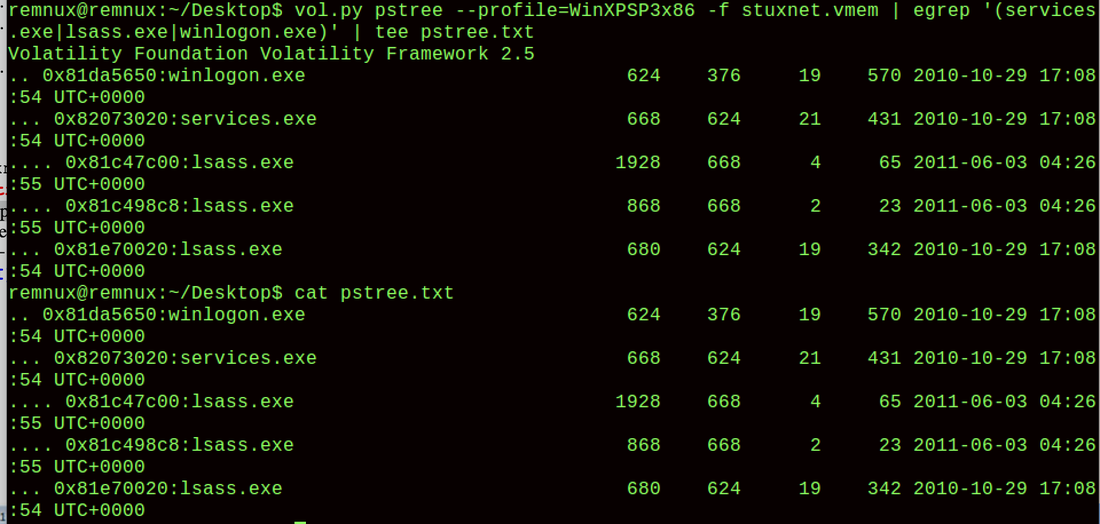
\includegraphics[width=0.49\textwidth]{images/STUXNET5.png}
	\caption{Stuxnet Process Tree}
	\label{fig:TCPIP}
\end{figure}



Dropper code of Stuxnet consist on a wrapper program that includes all of the above components stored inside itself in a section called “stub”. It is integral to the working of Stuxnet. When the malicious code is executed, the wrapper code extracts the .dll file from the stub section, maps it into memory of the OS as component of module, and calls one of the exports.
A pointer to the original stub section is transferd as a parameter. This process will export this time and then will extract the .dll file from the stub section code, which was passed as an instruction to be mapped  into memory and  then call another different process export from inside the previously mapped .dll file. The pointer code to the original stub section is then passed but this time as a parameter. This occurs continuously throughout the execution of the malicious code, so the original stub code inside this section is continuously passed between different functions and processes as parameters for the main payload. In this way every single layer of the threat is always accessed to the main .dll and the configuration blocks[12].
Additionally it loading the .dll file right into the memory to then call an export process directly, Stuxnet this worm also used some other techniques in order to call exports from the main .dll file. This techniques are read an executable template from its own resources, fill-out it with right data, like a .dll file to load and then export to a call, and then to inject this new executable template to another process for execute it then this new executable template will load the original .dll code file and will call whatever exports this template which was with the information it was populated.
Even if this threat uses two different techniques to call the exports into the main .dll file, it should be clear that all the functions of this threat can be proved by analyzing all of the exports from the main .dll file

\subsection{Exploitation}
Phase I: Propagation.

The Stuxnet penetrated to the target infrastructure with help of removable storage media such as USB drives. This kind of attack are mainly relying on human interaction to infect the virus from one system to another[13].  After infection, Windows operating system appears and manages shortcuts with the extensions '.lnk' and '.pif'. More precisely, the vulnerability relates to the way that the icon for the link is loaded. It was loaded through CPL (Windows Control Panel)
file using the system function 'LoadLibraryW()', a CPL file is just a DLL file.  By specifying the appropriate information as the access path to a malicious 'dll' in the section 'File Location Info' of a lnk file, this mechanism  forced  Windows operating system to execute arbitrary code by displaying the content of a directory.

Exploitation  requires only user to open and execute a malicious directory. Exploitation code can be created and published within the Metasploit framework. Then exploited system or user needed to get an Internet access then it was taken control of the  over infected remote system, then  server forces the infected client to open a shared file using the WebDAV protocol[14].

When  inspecting infected an USB flash drive with the Stuxnet worm, it contained inside 6 files:
\begin{itemize}
   \item  Copy of Shortcut to.lnk;
   \item  Copy of Copy of Shortcut to.lnk;
   \item  Copy of Copy of Copy of Shortcut to.lnk;
   \item Copy of Copy of Copy of Copy of Shortcut to.lnk;
   \item  Copy of Copy of Copy of Copy of Shortcut to.lnk;
   \item ~WTR4141.TMP;
   \item  ~WTR4132.TMP.
\end{itemize}

 After all, the Stuxnet does not only rely on help from users to spread in the system.  While it started to infect other services in the system which can be remotely exploited within a local network. The first was the Microsoft print spooler, while the second targets the old vulnerability presented within the server service (MS08-067). As we know that when a printer is shared on a system and local network, then any user is able to print, read and write files into the "System" directory. The exploitation of vulnerability was taken in two phases. The first was  inserting files "winsta.exe" and "sYsnuIlevnt.m0f" to the directories
"Windows\System32" and "Windows\System32\wbem
\mof". 
Finally, the Stuxnet exploited the old MS08-067 security vulnerability in the server service, which was massively exploited by Conficker Downadup. The main goal is to insert a file in shared directories of the' C:' or 'Admin:' directories. With using vulnerabilities of the task scheduler, it was executed in some special day by remote command. The shellcode used by the malware to execute two actions, as an advanced mechanism, in contrast, it was used by Conficker.



Phase II: installation of the malicious code.



 In order to ensure maximum dissemination and to be persistent, two security vulnerabilities are exploited by Stuxnet. 

The first vulnerability relates to the way the keyboard is managed by the driver "Win32k.sys". An index is loaded from a shared library without verification in order to force the system's kernel to execute code controlled from the user area network. 



The second vulnerability relates to the task scheduler.

Where is stored in an ordinary XML file
contained in the directory "SystemRoot\system32\Task". Access  is restricted there. To run changes in this directory,  the user is required a higher level of privileges, in order to elevate privileges.  After that, the Stuxnet adds a task which calculates the associated CRC32 hash, thus "manually" changes the file to raise the privileges associated with it, adds a comment field and fills it with random data to provoke a collision.The task is executed with the highest privileges.

\subsection{Functionality of malware}
In the USB drive execution of this module, it launches a rootkit. With the use of system functions associated with the shared libraries 'ntdll.dll' and 'kerneI32.dll' are intercepted so that code can be injected, and to hide the presence of various malicious files based on specific criteria ('.lnk' with a size of 1,471 bytes and 'WTRabcd.tmp' files for which the sum of a, b, c, and d modulo 10 is equal to 0).

The malware is capable of injecting executable code into running processes or into another process. These operations need not to load a file which cannot be detected by an antivirus program. Also, some network functionality were implemented within the malware: RPC client and server. Peer-to-Peer communications and the use of a C&C are mainly used to keep the malware up to date and to recover information, to download and install other malware or to exfiltrate or grab sensitive stolen information from the compromised system.



For maximizing the efficiency of the proliferation the operation, it seeks the WinCC software.

When it is discovered, Stuxnet connects to the
 database used by the software, using a standard hardcoded password, successfully connected to this database, the it sent the malicious code via SQL requests, then executes it locally.

It hid from plant personnel by installing rootkits on infected Windows computers and on infected PLCs, for hiding its files. By installing a driver on Windows computers, it hid by manipulating requests which were sent to devices. It intercepts calls from and to s7otbxdx.dll, then it hid the malicious code and it writes to PLCs to disrupt the functionality of centrifuges, and also protected its malicious codes from being overwritten by the system.

Before the malware run an attack routine, it records the centrifuges’ state as in normal operating frequencies and feeds this recorded data to the WinCC monitoring program during the attack. The result is that the system was in a normal operation state and not alerting monitoring system and personnel of the anomalies frequencies in the centrifuges.

Stuxnet also modified some functionality on the PLCs, in order to prevent a safe shutdown when the operator finds out that the system is operating abnormally.

%%%%%%%%%%%%%%%%%%%%%%%%%%%%%%%%%%%%%%%%%%%%%%%%
%continuar a alterar frases apartir daqui
\section{ Mechanism of Attacks on ICS/Scada.}
\label{sec:APP}
	In this section we cover some practical implementations that successfully transmitted data in a covert channel exploitation.
\subsection{Stages of executing of ICS attacks}

The first step in Stage 1 is called Reconnaissance. It has taken place prior to targeting the energy companies. However, the three impacted organizations analyses show they became targets due to their levels of automation in their distribution systems. Thus, it needs some period of time to be broken by the remote opening of breaches by breakers. Also, the targeting and final attack plan for
the targeted companies should be highly coordinated, which should indicate that reconnaissance will take place soon or some period of time. This stage can be seen as the diagram on Figure 5.

The second step is Weaponization and Targeting. Targeting normally take place when no weaponization is needed; all devices can be directly accessing through the internet, just scanning ports or it can be exposed through Shodan site. In this type of attack, the main goal is not targeting of specific infrastructure in order to gain access. Instead, the adversaries weaponized Microsoft Office documents (Excel and Word), mail, flash drive by embedding backdoor or worm within them. For example samples of Excel and other official documents have been recovered from the broader access campaign that targeted a majority of organizations in Ukraine, including Office documents used in the specific attack against the three

electricity companies. Which can be installed on the system, then run there locally.

Enabling the attachments allowed the malware to Exploit system functionality to install backdoor or worm on the victim system. The goal of using available functionality in the system is present throughout the kill chain of the adversary.

\begin{figure}[!htb]
	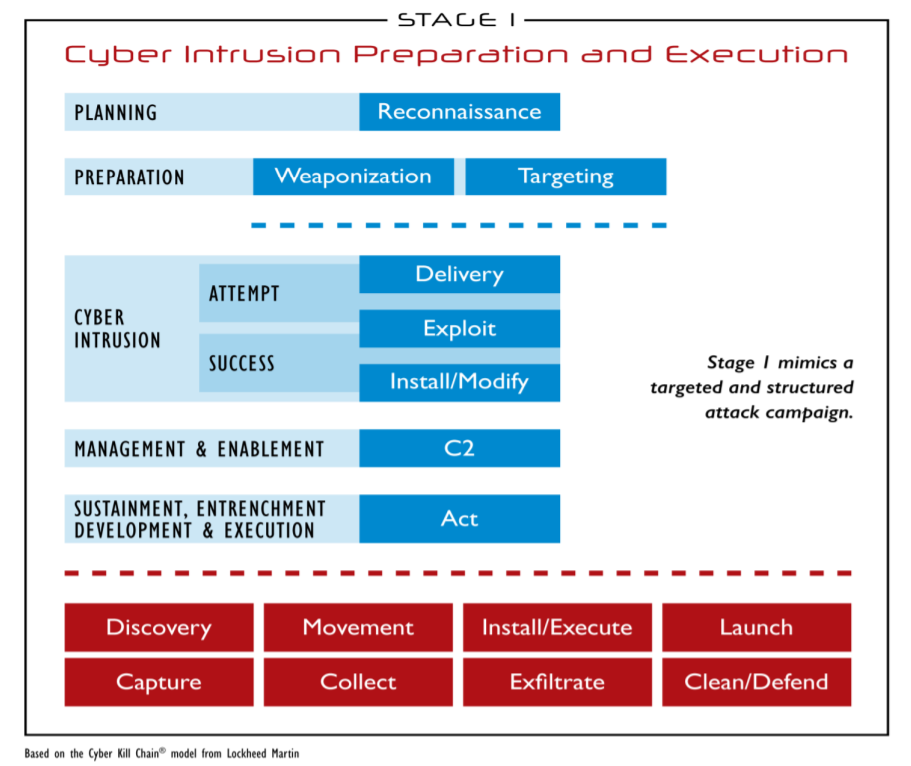
\includegraphics[width=0.49\textwidth]{STAGE1.png}
	\caption{ Stage 1- Cyber Intrusion preparation and Execution }
	\label{fig:TCPIP}
\end{figure}

 the Develop stage occurs in the adversary’s networks, and there should limit any available forensic
information gathering procedures, and the attack that follows this stage can not be revealed  about the adversarial process.
\begin{figure}[!htb]
	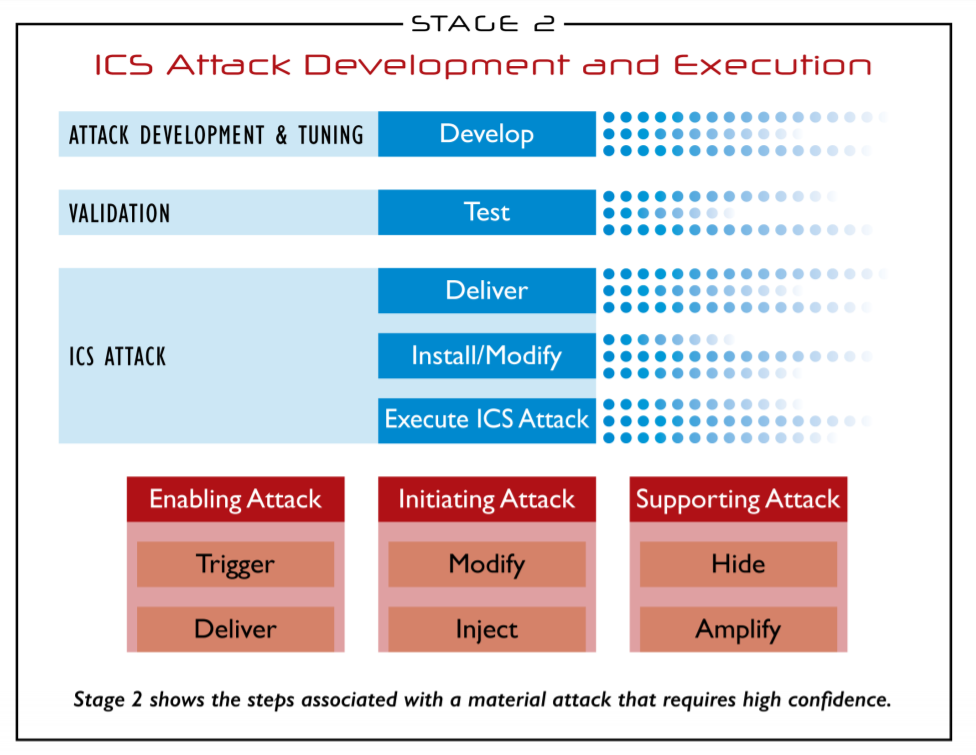
\includegraphics[width=0.49\textwidth]{STAGE2.png}
	\caption{ Stage 2- Attack Development and Execution }
	\label{fig:TCPIP}
\end{figure}

In Stage 2, in Figure 7, there are the Attack

Development and Tuning Stages, the hackers execute the Develop step in at least in two ways. The first way, they learn how to interact with the three distinct Distribution Management System(DMS) environments using the native control presented in the system, server, and operator desktop. The second way, developing malicious firmware, backdoors, worms or other tools for infecting and infiltrating the system and network devices.

The malicious firmware tools should be consistent among devices and then need to be uploaded within a short period of time into multiple sites, prior to the main attack for quick and predictable execution it in the local site. 

Finally, to complete the ICS Cyber Kill Chain and to execute the ICS Attack there, the adversaries should use the HMIs in the SCADA environment to open the breakers and run malware.	
	
\begin{figure}[!htb]
	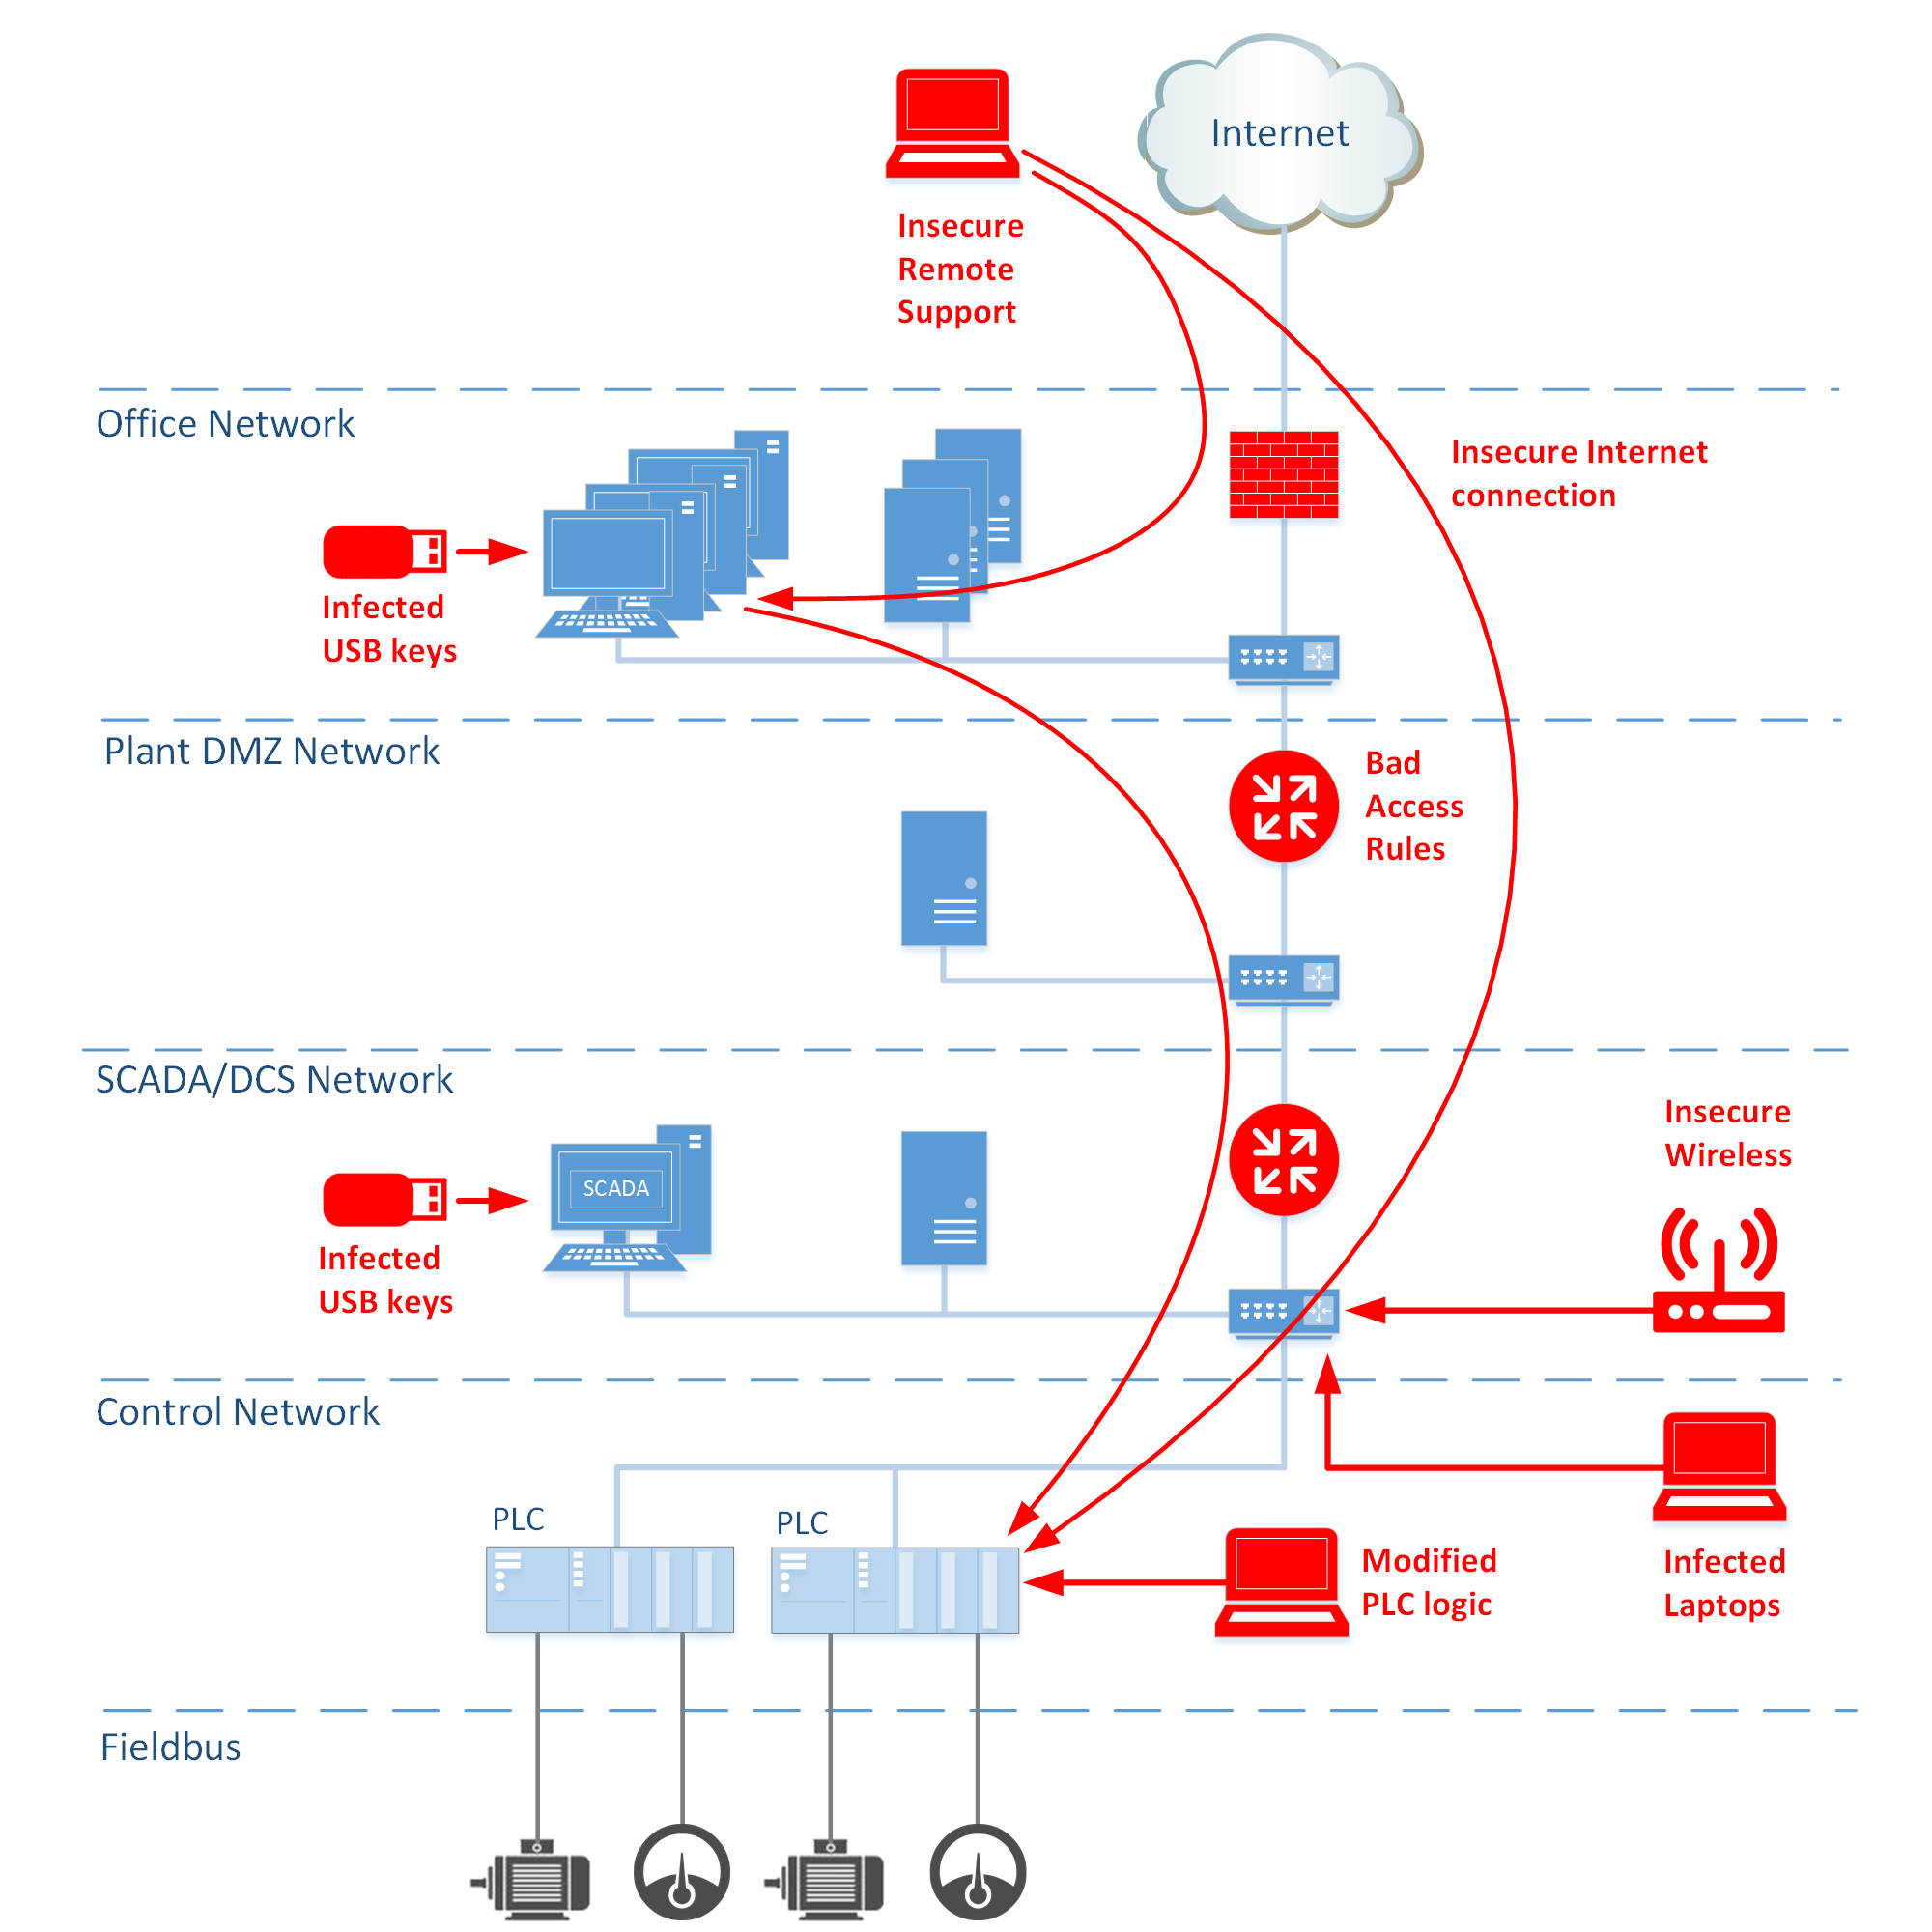
\includegraphics[width=0.49\textwidth]{images/SCADAATACK.png}
	\caption{Mechanism of Attacks %(from \cite{FACECAT})
	}
	\label{fig:fb}
\end{figure}

%%%%%%%%%%%%%%%%%%%%%%%%%%%%%%%%%%%%%%%%%%%%%%%%
%continuar a alterar frases apartir daqui
\section{Imitation  of  exploitation  on  new  version  of ICS/SCADA system}
\label{sec:APP}
For the experiment of exploitation, we used real-world ICS system image from the Gas Processing plant, which is Windows XP SP3 with Siemens Simatic software. We use Metasploit from Kali Linux OS and SANS Forensics tool for investigating worm. In this labs experiment, we compare features of use Windows XP and the newest version of Microsoft product. It will be pre upgrading procedures to prove that upgrading OS with new patches, it is very vital for the whole ICS system.

    Tools:

     Kali linux OS

     SANS SIFT OS

\subsection{Preparation}
In this stage we have just simulated the passive attack and used a simulation of USB flash drive in Metasploit, directly infect the system for Windows XP, Windows 7 and Windows Server 2012 R2 with latest updates and security patches.  

The main structure of this malware that it consists of both user-mode and kernel-mode components. In the user-mode functions were designed to do several things: 

1) chosen process injection - adding into a running process of OS, resulting of the execution of code in the target process’s address space;

2) checking suitable OS platform; 

3) escalating privileges of OS; 

4) install two kernel-mode drivers: for running Stuxnet after rebooting and rootkit to hide its files(see Figure 9). 

We have used the Metasploit framework to exploit some main vulnerabilities that Stuxnet uses. We have used console interface of the Metasploit framework called as msfconsole.
\begin{figure}[!htb]
	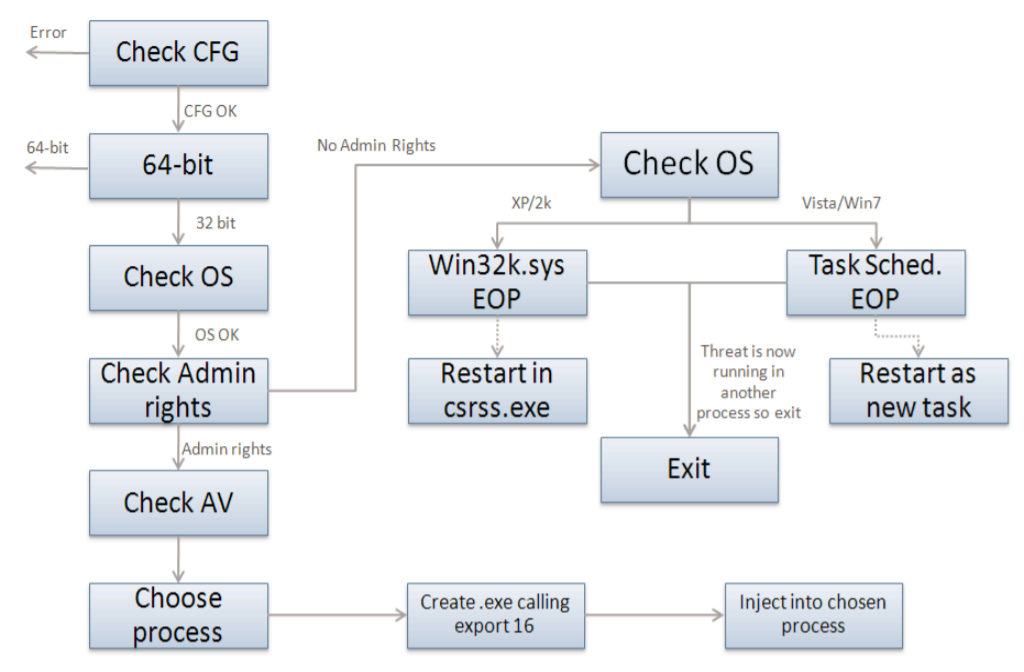
\includegraphics[width=0.49\textwidth]{images/process.png}
	\caption{ Stuxnet control flow %(from \cite{FACECAT})
	}
	\label{fig:fb}
\end{figure}


\subsection{Infection from user: Windows XP based Siemens Simatic}

The main module DLL exports 21 functions (see in Figure 10). Stuxnet starts by calling export 15. In this function, it starts to check if it is running on a suitable Windows OS version. Assuming it is and the machine or server is not exploited, it uses  zero-day exploits, which depends on the version of Windows OS, to gain its privileges.


\begin{figure}[!htb]
	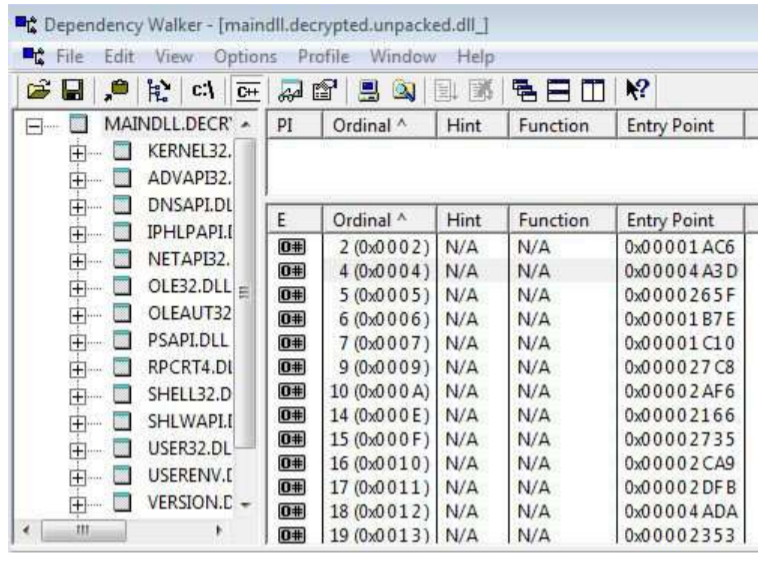
\includegraphics[width=0.49\textwidth]{images/walker.png}
	\caption{ Stuxnet’s main library export functions as shown by Dependency Walker %(from \cite{FACECAT})
	}
	\label{fig:fb}
\end{figure}


Export 16 used then call an installation: it injects code into the services.exe process in order to infect removable USB drives and any Step7  projects it finds. 

\begin{figure}[!htb]
	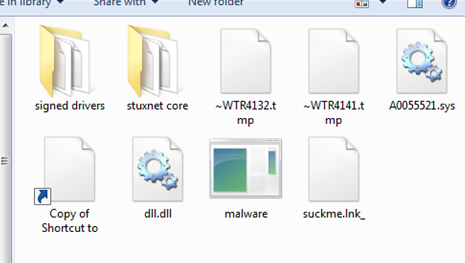
\includegraphics[width=0.39\textwidth]{images/STUXNET1.png}
	\caption{Infected USB flash drive %(from \cite{FACECAT})
	}
	\label{fig:fb}
\end{figure}

Upon execution, Stuxnet creates two drivers on the compromised machine, called mrxcls.sys and mrxnet.sys which were installed in kernel[19]. The drivers are used to mask the malware on both the USB drive and the infected PC(see on Figure 11). They were are signed using the Realtek certificate. The program doesn’t seem to do anything else malicious after it’s on a new machine, although it will copy itself to other USB drives attached to the PC. It will drop two driver files to install the driver files, Mrxnet.sys and Mrxcls.sys and signed with a certificate from a company called "JMicron Technology Corp" (see on Figure 12).
\begin{figure}[!htb]
	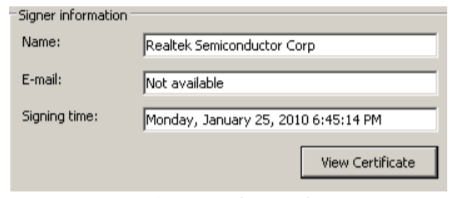
\includegraphics[width=0.49\textwidth]{images/realtek.PNG}
	\caption{ Digital Signature Information from MRXCLS.sys %(from \cite{FACECAT})
	}
	\label{fig:fb}
\end{figure}

\subsection{Infection from user: EternalSynergy}

Injections  will not work when you are trying to inject a DLL from 64-bit processes into 32-bit processes or vice versa, due to the Windows-on-Windows for 64-bit (WoW64) kernel. The 64-bit processes require pointers that are 64 bits so the pointer we passed to CreateRemoteThread() for LoadLibrary() would need to be a 64-bit pointer. Though our injection application was 32 bits, we could not specify a 64-bit pointer in it.



So we go to the web resource Exploit-DB. Under the Remote Code Execution Exploits section, we can find the exploit under its Microsoft x64 designation, MS17-010 which called as Microsoft Windows -"EternalRomance"/"EternalSynergy"/"EternalChampion" SMB Remote Code Execution (Metasploit) (MS17-010) vulnerability is already patched by Microsoft;

it allows arbitrary code execution from SMB clients sending specially malformed path strings[20][21].

We used this vulnerability to get access to network shares like shared folders on the LAN and when any machine on the LAN accesses this folder, Stuxnet files get copied to that machine and hide [22].
\begin{figure}[!htb]
	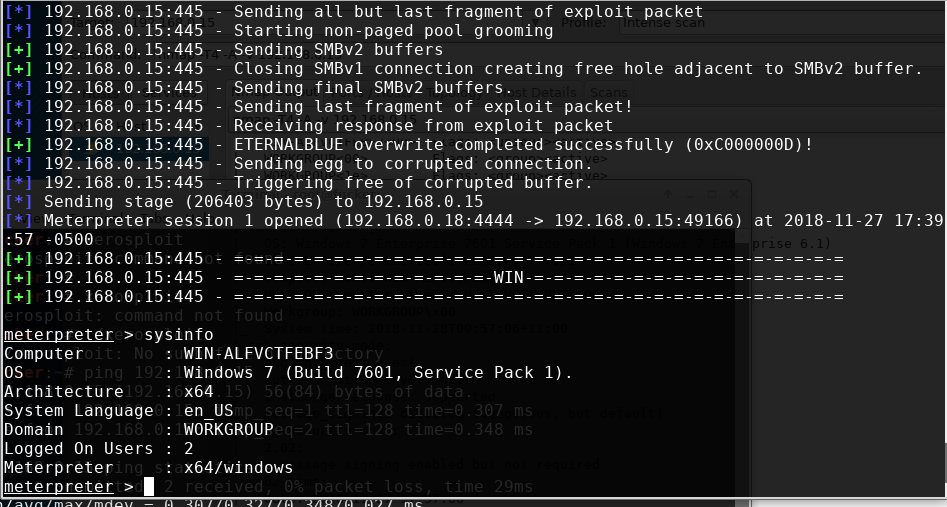
\includegraphics[width=0.49\textwidth]{images/eternalblue.png}
	\caption{ SMB Remote Code Execution}
	\label{fig:fb}
\end{figure}

the exploit  allowed us to execute code on Windows machines with SMB services exposed to external connections, see on Figure 14.

\begin{figure}[!htb]
	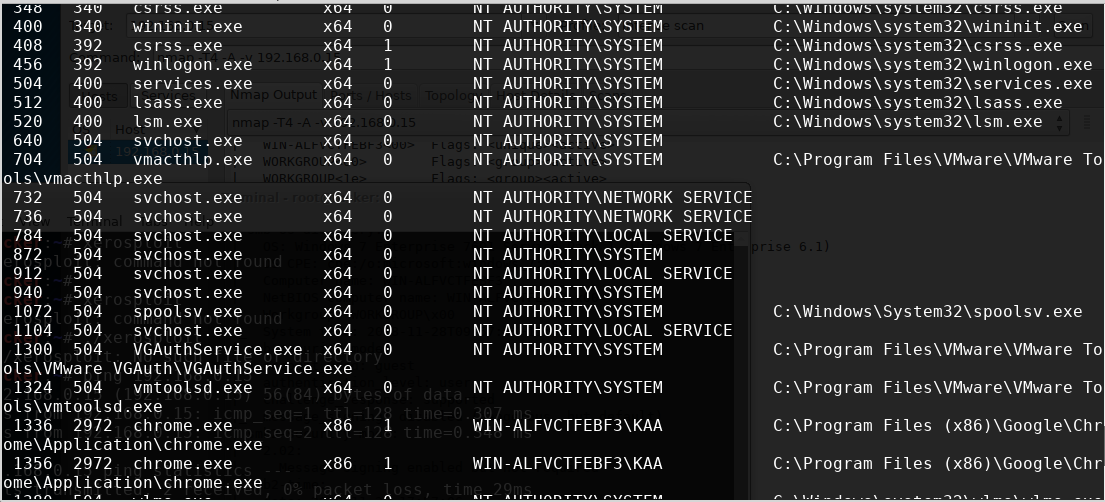
\includegraphics[width=0.49\textwidth]{images/svhostexe.png}
	\caption{ Listing processes on attacked machine	}
	\label{fig:fb}
\end{figure}

\subsection{Infection from user: Exploit with DoublePulsar}

DoublePulsar is an implant leaked by the ShadowBrokers group last year that enables the execution of additional malicious code. It was commonly delivered by the EternalBlue exploit and was the most famous from its recent use to deploy the Wanna Decryptor 2.0 (WannaCry) ransomware. Even with industry leading AV, IDS, and VM solutions, DoublePulsar attacks had been proven difficult to prevent and detect[].

SMB version 1 (SMBv1) in various versions of Microsoft Windows accepted specially crafted packets from remote attacker machine, this vulnerability allows us to perform Remote Code Execution which was particularly targeted our Windows 7 and XP.



After installation DOUBLEPULSAR  waits for certain types of data to be sent over port 445. When DOUBLEPULSAR  arrives, the implant provides a distinctive response(see in Figure 15 and 16).

\begin{figure}[!htb]
	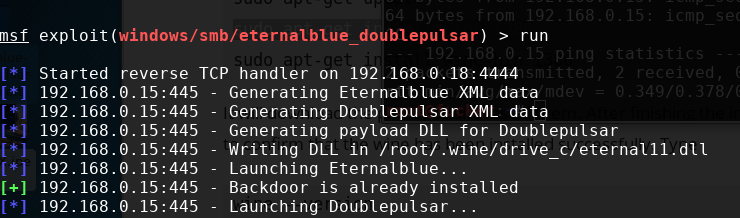
\includegraphics[width=0.49\textwidth]{images/injectiondb.png}
	\caption{Creating backdoor}
	\label{fig:fb}
\end{figure}
 Once DoublePulsar is on a compromised host, we could drop additional malware or executables onto a machine, meaning that this bug will quickly move from the exclusive realm of nation-state hackers to cybercriminals, and it might be a matter of time before ransomware and other commodity malware and botnets take advantage of these exploits to spread.
 \begin{figure}[!htb]
	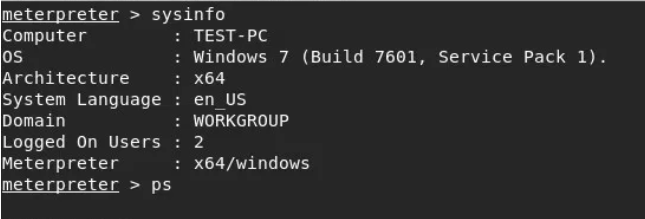
\includegraphics[width=0.49\textwidth]{images/insidedb.png}
	\caption{Inside the OS}
	\label{fig:fb}
\end{figure}
 
 
 


\subsection{Conclusion:}
For carrying out Stuxnet simulation, following
assumptions have been made.
Stuxnet initial propagation is through USB, we used  Metasploit framework as act of using USB and exploitation takes place through this. Also we have exploited it with svchost.exe and stuxnet.exe processes which loaded into system where we could connect remotely there through Windows RDP, installing privileged user accounts in MSSQL and into OS.

%%%%%%%%%%%%%%%%%%%%%%%%%%%%%%%%%%%%%%%%%%%%%%%%%%%%%%%%



\section{Invistigate of Vulnerabilities in critical infrastructure in this type of attacks.}
\label{sec:CM}
The last cyber attacks performed against Ukrainian oblenergos were well planned and highly coordinated. The attacks can consist of several major elements with both enabling and supporting attack segments. The attackers can be remote and can interact with multiple locations within each of their targets. Distribution utilities traditionally have both central business and engineering offices and a number of branch facilities used to bring support to line staff, meter reading, bill payment, and distributed supervisory control operations. Some types of cyber attacks designed to maliciously taking over and operating an SCADA DMS may be best implemented in a distributed way at the lowest or most direct level (from a local sending and SCADA server out of the substations that are being monitored and controlled).
\begin{figure}[!htb]
	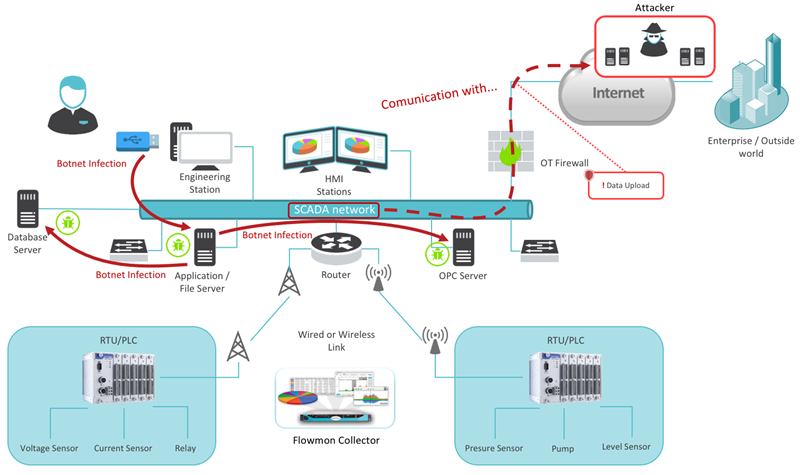
\includegraphics[width=0.49\textwidth]{images/infiltration2.png}
	\caption{Exploitation to the ICS infrastructure }
	\label{fig:fb}
\end{figure}

Preparing for  multifaceted
attack is not easy and it requires careful planning, testing, with integrated defense(active and passive), and some operations exercises which related to industries.
The next attack may purposefully differ in its approach to throw off or defeat the defender’s plans and expectations, example on Figure 17. It is critical that defenders exercise and train against different possible scenarios and to be aware of the possible attackers and know who they possibly are co-actively and creatively. It is vital to develop capabilities with flexibility in mind.


\subsection{Define proper architecture and preventions}
A common way to think is that ICS and SCADA networks are physically separated from corporate IT networks. This might be accurate physically, in the sense that some companies operate distinct LANs or air gap their control and corporate networks  from one another. In other cases, companies use the same LANs and WANs but encrypt their ICS and SCADA traffic across a shared infrastructure. More frequently, however, networks require some level of interconnectivity in order to obtain operational input from addition or export data to external 3rd party systems. 

In order to eliminate anomaly traffic in infrastructure need control these entities:
\begin{itemize}
\item Host Security
\item Network Security
\item Traffic Normalization
\end{itemize}


	While host security may prevent the channel's exploitation in some situations, protecting hosts from directed attacks, it cannot remove covert network channels. For example, and citing from: "If the hosts are secured in order to avoiding to being hacked, hackers cannot exploit covert channels. However, this does not protect against data ex-filtration by insiders, nor does it solve the problem of covert channel in other scenarios such as censorship circumvention".



	However, network security is possible to resist tunneling channels by blocking susceptible protocols and traffic. One example is the firewall blockage to Internet Control Message Protocol (ICMP). Nonetheless, there are protocols on the Internet that cannot be blocked, given their importance. Each traffic should be under control.



	In regard to traffic normalization, by normalizing protocol headers, header extensions, and padding, can mitigate simple storage covert channels.
	
	
\subsection{SECURING ICS AND SCADA PROCESSES}	

This section suggests guidelines for protecting ICS and SCADA infrastructures through procedures for preventing and stop intruders and analysis of the security risks and implementing a comprehensive security strategy to hardening infrastructure assets.

	

Firstly, need	properly segment networks from each other.
By ensuring that logging is enabled on devices and can support it, including both ICT and Operational Technology (OT)assets.

All devices in network architecture(switches, routers and etc) are managed and have the ability to capture data from the network in order to support Passive and Active Defense mechanisms, an example in Figure 18.

Need to make backups of critical software installers and including theirs an MD5 and SHA256 digital hash of the installers.

Be sure that backup project files are collected and vaulted from the network.

Need periodically test the tools and technologies that passively and actively defend and to achieve that which mechanisms will be needed (such as digital imaging software) on the environment in order to ensure that it will not negatively impact on the local systems. Prioritize and patch assets(OS, network devices) against vulnerabilities based on the most critical CVE.

Also should be limited remote connections only to personnel that need them with use of two-form authentication on the remote connections. Should be used system event monitoring system, configured and monitored specifically for high-value ICS/SCADA systems.

\begin{figure}[!htb]
	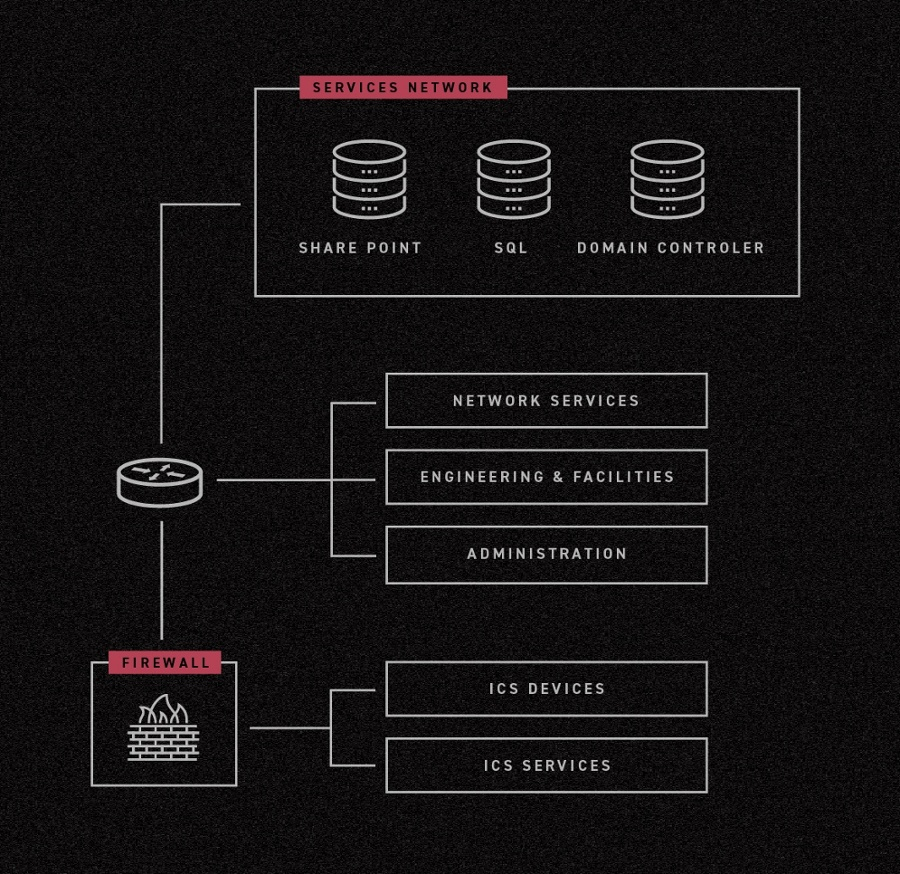
\includegraphics[width=0.49\textwidth]{images/Str_scada.jpg}
	\caption{ICS  infrastructure: Application and hardware }
	\label{fig:fb}
\end{figure}

Also, need to implement Policy for Application whitelisting which can help limit adversary initial infection vectors and should be used when whit an approach not too invasive to the ICSs.

Critically need that DMZs and properly tuned firewalls between network segments will give visibility into the environment and allow defenders(asset owners) the time required to identify intrusions and localize it.

For that purpose also need to establish a central system for logging and data aggregation used as point to allow forensic evidence to be collected and made available to defenders. Implementation of alarm package priorities for abnormal cyber events within the control system. For user and part need to enforce a password reset policy in the event of a compromise one especially speaking for VPNs and administrative accounts. Need periodically update antivirus and endpoint security technologies to allow for the detection of known malware. Also should be configured an intrusion detection system so that rules can be deployed fast to search for intruders.



The personnel need to provide pieces of training for detecting and  hunting for odd communications leaving the networked environment such as new IP
communications.

Perform network security monitoring to continuously search through the networked environment for abnormalities.Need to plan and train to incident response plans that integrates both the IT and OT network personnel and consider active defense models for security operations such as the active cyber defense cycle. It also should be better to ensure that personnel performing analysis have access to technologies such as sandboxes to quickly analyze incoming phishing emails or odd files and extract indicators of compromise (IOCs) to search for infected systems. And for that purpose use backup and recovery tools to take digital images from some of the systems in the supervisory environment such as HMIs and data historian systems every 6-12 months. This will allow a baseline of activity to be constructed and make the available the images for scanning with new IOCs like as new YARA rules on emerging malicious threats or other forensic tools and train them on using forensic tools such as YARA to scanning digital images and also evidence collected from the environment but do not perform the scans in the production environment itself.

Good architecture and passive defense practices build a defensible ICS; active defense processes establish a defended ICS environment. Countering flexible and persistent human adversaries requires properly trained and equipped human personnel[9].




\section{Conclusion}
 Over the last couple of years, Iran became the main player in offensive cyber operations, especially targeting US critical infrastructure, second only to Russia. The problem with these intrusions is that virtually nobody has a good idea which damage they can cause if it would be activated. If some countries cyber operations have succeeded at anything, it is the creation of a credible deterrent.



As traditional corporate IT perimeters have disappeared, as corporate and operational systems have become more thoroughly integrated, and as organizations leverage the continuing emergence of new technologies, cyber threats will continue to evolve. Cyber risks are often changing fast changing than companies can react on it, and cyberattacks are more frequent, sophisticated, and malicious. To achieve their growth and innovation potential, company executives, business owners, and ICT management need to make integral investment in cyber-risk assessment capabilities. 

Stuxnet poses a significant threat to a vulnerable infrastructure. Stuxnet’s repository code is available to anyone with connection to internet and could be reused and modified again with variable amounts of efforts against something. Computer hackers, foreign intelligence services, organized crime, and terrorists are just a few potential suspects that the some of countries recognize as persons or groups who may make use of Stuxnet’s code for carrying out a cyber-attack against any specific countries.

Through these damages, any number of evil goals might be achieved. For instance, for military purposes, this kind of attacks could be used as first strike weapon –covertly compromising a target before an overt offensive. Also, such an attack could be used to cause political and region instability and  fear. If a government is unable to support security and essential services, the result would be dramatic and a loss of public confidence and fear of further cyberattacks. Thus solutions must be investigated and implemented in these critical infrastructures. To prevent sources of threats from criminal groups, hackers, terrorists, an organization in such a situation and grant stability on the country.


    
% references section

%\bibliography{covert}{}
%\bibliographystyle{plain}
\begin{thebibliography}{1}

\bibitem{}
D. Bailey, E. Wright, “Practical SCADA For Industry, ISBN 9780750658058, Newnes, 2003

\bibitem{}
 R. Kalapatapu, “SCADA Protocols and Communication Trends”, ISA EXPO, 2004

\bibitem{}
Falco, Joe, etal., IT Security for Industrial Control Systems, NIST IR 6859, 2003,http://www.isd.mel.nist.gov/documents/falco/
ITSecurityProcess.pdf.  

\bibitem{}
 T. Morris, R. Vaughn, Y. Dandass, “A Testbed for SCADA
Control System Cybersecurity Research 
and Pedagogy”, In proceedings of the Seventh Annual Workshop on Cyber Security and Information 
Intelligence Research (CSIIRW '11), 2011, Oak Ridge, Tennessee, USA
\bibitem{}
Beale, J., Baker, A., Esler, J., Kohlenberg, T., and Northcutt,
S. (2007). Snort: IDS and IPS Toolkit. Jay Beale’s
open source security series. Syngress.
\bibitem{}
Deng, Y. and Shukla, S. (2013). A distributed real-time
event correlation architecture for SCADA security. In
Critical Infrastructure Protection VII, volume 417 of
IFIP Advances in Information and Communication
Technology, pages 81–93. Springer Berlin Heidelberg.
http://dx.doi.org/10.1007/978-3-642-45330-4 6.
\bibitem{}
Morris, T. H. and Gao, W. (2013).
Industrial
control system cyber attacks.
In Proceed-
ings of the 1st International Symposium for
ICS & SCADA Cyber Security Research.
http://ewic.bcs.org/content/ConWebDoc/51165.
\bibitem{}
Wilamowski, B. M. and Irwin, J. D. (2011). The Indus-
trial Electronics Handbook – Industrial Communica-
tions Systems, volume 2 of The Industrial Electronics
Handbook. CRC Press, Taylor & Francis Group, 2
edition.
\bibitem{}
Joiner, K., E. Sitnikova and M. Tutty, ‘Structuring defence
cyber-survivability T&E to research best practice in cyber-
resilient systems’, paper presented at Systems Engineering
Test and Evaluation Conference, Melbourne, 2016, available
at http://search.informit.org/documentSummary;dn=
255735974744392;res=IELENG accessed 23 June 2017
\bibitem{}
Office of the Secretary of Defense, ‘Procedures for operational
test and evaluation of cybersecurity in acquisition programs’,
memorandum dated 1 August 2014, available at  http://www.
dote.osd.mil/pub/policies/2014/8-1-14\_Procs\_for\_OTE\_of\_
Cybersec\_in\_Acq\_Progs(7994).pdf  accessed 30 May 2017.

\bibitem{}
 The website of isis. Technical report, World Wide Web, http://www.isis-online.org.
\bibitem{}
David Albright, Paul Brannan, and Christina Walrond. Did stuxnet take out 1,000 centrifuges
at the natanz enrichment plant? Technical report, World Wide Web, http://isis-online.
org/uploads/isis-reports/documents/stuxnet\_FEP\_22Dec 2010.pdf, December 2010
\bibitem{}
Mark Clayton. Stuxnet cyberweapon looks to be one on a production line, researchers
say. Technical report, World Wide Web, http://www.csmonitor.com/USA/2012/0106/
Stuxnet-cyberweapon-looks-to-be-one-on-a-production-line-researchers-say,
January 2012
\bibitem{}
Nicolas Falliere, Liam O Murchu, and Eric Chien. W32.stuxnet dossier (version 1.4). Technical
report, World Wide Web, http://www.symantec.com/content/en/us/enterprise/media/
security\_response/whitepapers/w32\_stuxnet\_dossier.pdf, February 2011.
\bibitem{}
Kim Zetter. How digital detectives deciphered stuxnet, the most menacing malware in history.
Technical report, World Wide Web, http://www.wired.com/threatlevel/2011/07/
how-digital-detectives-deciphered-stuxnet/all/1, 2011
\bibitem{}
Wikipedia. Simatic s5 plc. Technical report, World Wide Web, http://en.wikipedia.org/
wiki/Simatic\_S5\_PLC/, February 2012
\bibitem{}
The web site Triton vulnerability https://ics.sans.org/media/E-ISAC\_SANS\_Ukraine\_DUC\_5.pdf
\bibitem{}
Attackers Deploy New ICS Attack Framework “TRITON” and Cause Operational Disruption to Critical Infrastructure, web site resource https://www.fireeye.com/blog/threat-research/2017/12/attackers-deploy-new-ics-attack-framework-triton.html
\bibitem{}
https://www.esetnod32.ru/company/viruslab/ analytics/doc/Stuxnet\_Under\_the\_Microscope.pdf
\bibitem{}
How to use a reverse shell in Metasploit, link 
https://github.com/rapid7/metasploit-framework/wiki/How-to-use-a-reverse-shell-in-Metasploit
\bibitem{} About Eternal- Energy Exploit, web link
https://blogs.technet.microsoft.com/srd/2017/07/13/eternal-synergy-exploit-analysis/
\bibitem{}
https://hitcon.org/2017/CMT/slide-files/d2\_s2\_r0.pdf
\end{thebibliography}
\bibliographystyle{plain}

\end{document}